Like any accelerator architecture, predicting when an FPGA is the right choice of accelerator vs. an alternative often comes down to knowledge of the architecture, the application characteristics, and the system bottlenecks. This section describes some of the characteristics of an application to consider.\par

\hspace*{\fill} \par %插入空行
\textbf{Lots and Lots of Work}

Like most modern compute accelerators, achieving good performance requires a large amount of work to be performed. If computing a single result from a single element of data, then it may not be useful to leverage an accelerator at all (of any kind). This is no different with FPGAs. Knowing that FPGA compilers leverage pipeline parallelism makes this more apparent. A pipelined implementation of an algorithm has many stages, often thousands or more, each of which should have different work within it in any clock cycle. If there isn’t enough work to occupy most of the pipeline stages most of the time, then efficiency will be low. We’ll call the average utilization of pipeline stages over time occupancy of the pipeline. This is different from the definition of occupancy used when optimizing other architectures such as GPUs!\par

There are multiple ways to generate work on an FPGA to fill the pipeline stages, which we’ll cover in coming sections.\par

\hspace*{\fill} \par %插入空行
\textbf{Custom Operations or Operation Widths}

FPGAs were originally designed to perform efficient integer and bitwise operations and to act as glue logic that could adapt interfaces of other chips to work with each other. Although FPGAs have evolved into computational powerhouses instead of just glue logic solutions, they are still very efficient at bitwise operations, integer math operations on custom data widths or types, and operations on arbitrary bit fields in packet headers.\par

The fine-grained architecture of an FPGA, described at the end of this chapter, means that novel and arbitrary data types can be efficiently implemented. For example, if we need a 33-bit integer multiplier or a 129-bit adder, FPGAs can provide these custom operations with great efficiency. Because of this flexibility, FPGAs are commonly employed in rapidly evolving domains, such as recently in machine learning, where the data widths and operations have been changing faster than can be built into ASICs.\par

\hspace*{\fill} \par %插入空行
\textbf{Scalar Data Flow}

An important aspect of FPGA spatial pipelines, apparent from Figure 17-4, is that the intermediate data between operations not only stays on-chip (is not stored to external memory), but that intermediate data between each pipeline stage has dedicated storage registers. FPGA parallelism comes from pipelining of computation such that many operations are being executed concurrently, each at a different stage of the pipeline. This is different from vector architectures where multiple computations are executed as lanes of a shared vector instruction.\par

The scalar nature of the parallelism in a spatial pipeline is important for many applications, because it still applies even with tight data dependences across the units of work. These data dependences can be handled without loss of performance, as we will discuss later in this chapter when talking about loop-carried dependences. The result is that spatial pipelines, and therefore FPGAs, are compelling for algorithms where data dependences across units of work (such as work-items) can’t be broken and fine-grained communication must occur. Many optimization techniques for other accelerators focus on breaking these dependences though various techniques or managing communication at controlled scales through features such as sub-groups. FPGAs can instead perform well with communication from tight dependences and should be considered for classes of algorithms where such patterns exist.\par

\begin{tcolorbox}[colback=blue!5!white,colframe=blue!75!black, title=LOOPS ARE FINE!]
A common misconception on data flow architectures is that loops with either fixed or dynamic iteration counts lead to poor data flow performance, because they aren’t simple feed-forward pipelines. At least with the Intel DPC++ and FPGA toolchains, this is not true. Loop iterations can instead be a good way to produce high occupancy within the pipeline, and the compilers are built around the concept of allowing multiple loop iterations to execute in an overlapped way. Loops provide an easy mechanism to keep the pipeline busy with work!
\end{tcolorbox}

\hspace*{\fill} \par %插入空行
\textbf{Low Latency and Rich Connectivity}

More conventional uses of FPGAs which take advantage of the rich input and output transceivers on the devices apply equally well for developers using DPC++. For example, as shown in Figure 17-6, some FPGA accelerator cards have network interfaces that make it possible to stream data directly into the device, process it, and then stream the result directly back to the network. Such systems are often sought when processing latency needs to be minimized and where processing through operating system network stacks is too slow or needs to be offloaded.\par

\hspace*{\fill} \par %插入空行
Figure 17-6. Low-latency I/O streaming: FPGA connects network data and computation tightly
\begin{center}
	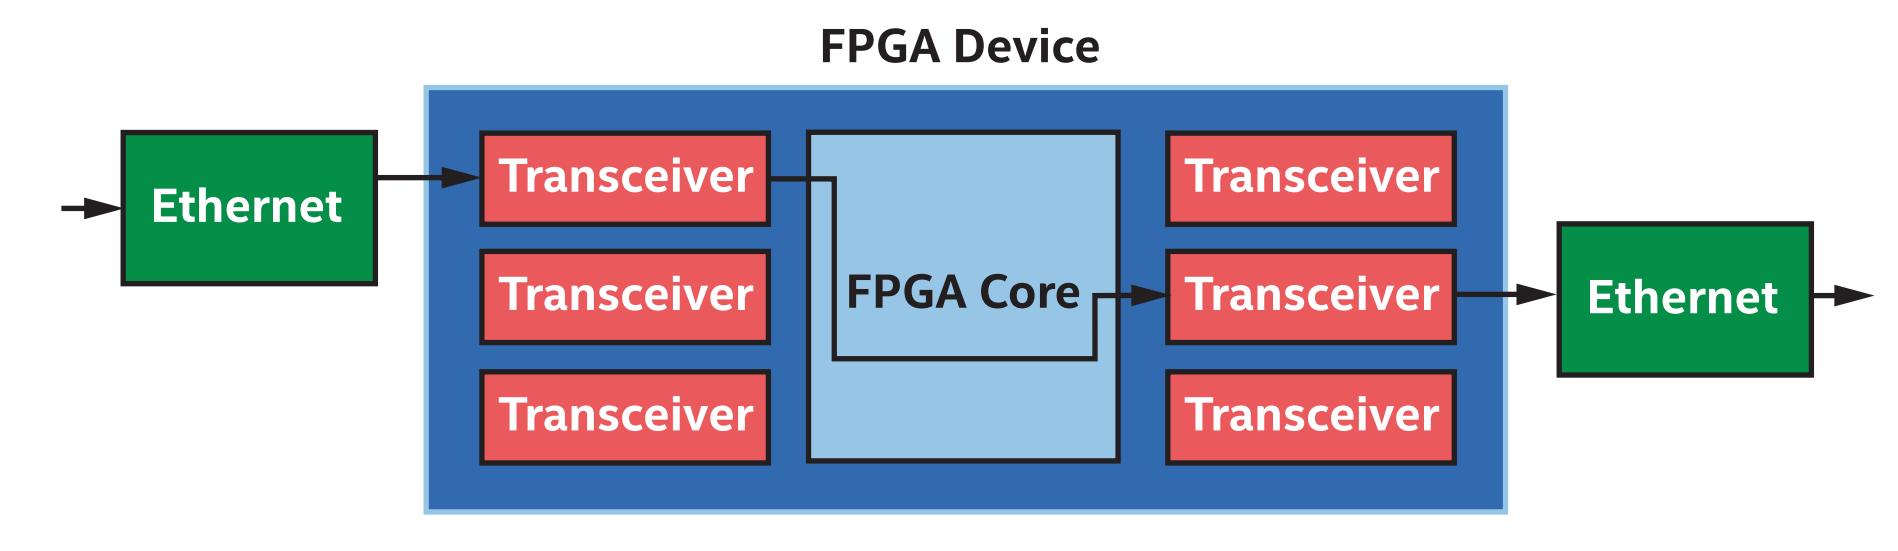
\includegraphics[width=1.0\textwidth]{content/chapter-17/images/7}
\end{center}

The opportunities are almost limitless when considering direct input/output through FPGA transceivers, but the options do come down to what is available on the circuit board that forms an accelerator. Because of the dependence on a specific accelerator card and variety of such uses, aside from describing the pipe language constructs in a coming section, this chapter doesn’t dive into these applications. We should instead read the vendor documentation associated with a specific accelerator card or search for an accelerator card that matches our specific interface needs.\par

\hspace*{\fill} \par %插入空行
\textbf{Customized Memory Systems}

Memory systems on an FPGA, such as function private memory or workgroup local memory, are built out of small blocks of on-chip memory. This is important because each memory system is custom built for the specific portion of an algorithm or kernel using it. FPGAs have significant on-chip memory bandwidth, and combined with the formation of custom memory systems, they can perform very well on applications that have atypical memory access patterns and structures. Figure 17-7 shows some of the optimizations that can be performed by the compiler when a memory system is implemented on an FPGA.\par

\hspace*{\fill} \par %插入空行
Figure 17-7. FPGA memory systems are customized by the compiler for our specific code
\begin{center}
	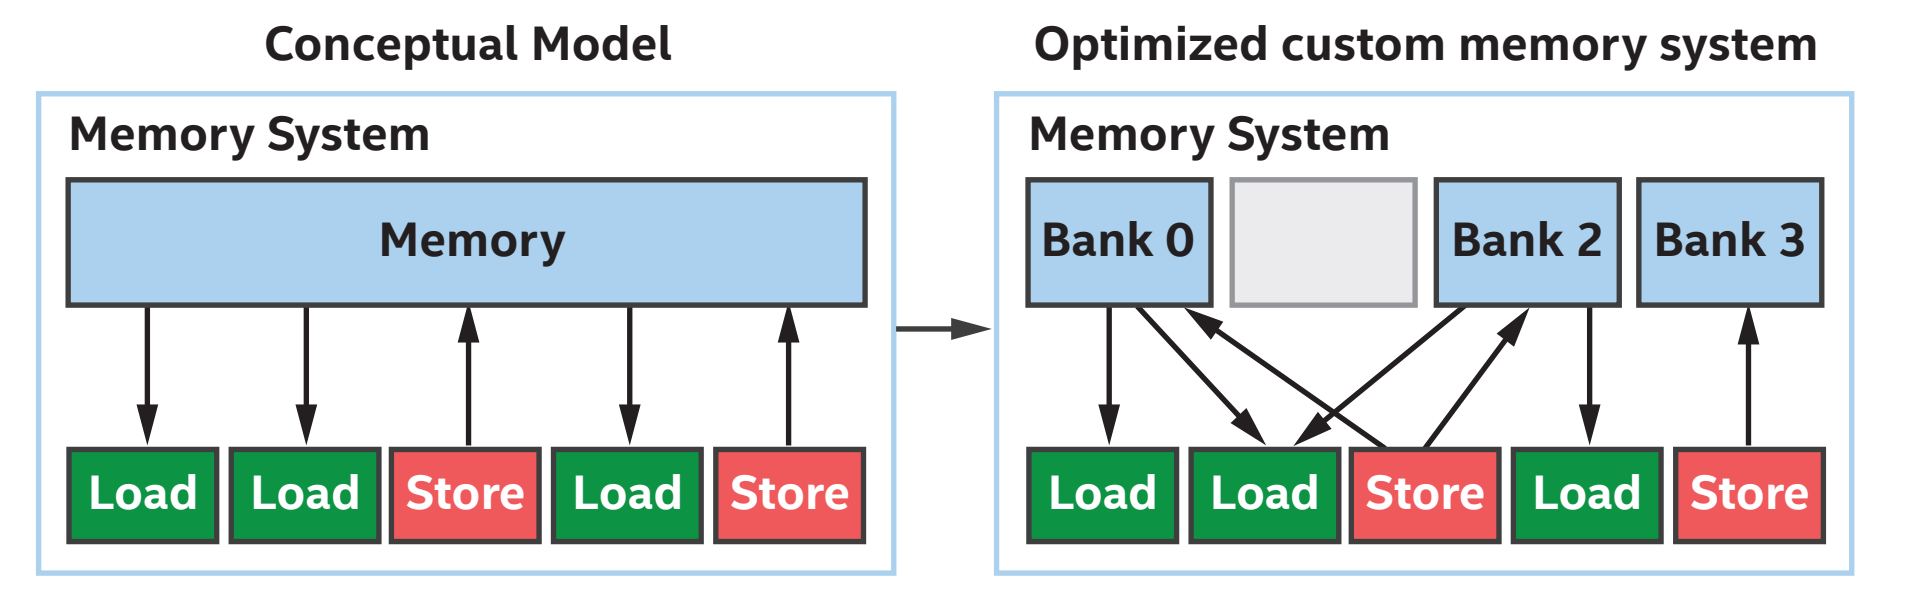
\includegraphics[width=1.0\textwidth]{content/chapter-17/images/8}
\end{center}

Other architectures such as GPUs have fixed memory structures that are easy to reason about by experienced developers, but that can also be hard to optimize around in many cases. Many optimizations on other accelerators are focused around memory pattern modification to avoid bank conflicts, for example. If we have algorithms that would benefit from a custom memory structure, such as a different number of access ports per bank or an unusual number of banks, then FPGAs can offer immediate advantages. Conceptually, the difference is between writing code to use a fixed memory system efficiently (most other accelerators) and having the memory system custom designed by the compiler to be efficient with our specific code (FPGA).\par



























